
\begin{figure*}[ht!]
	\centering
	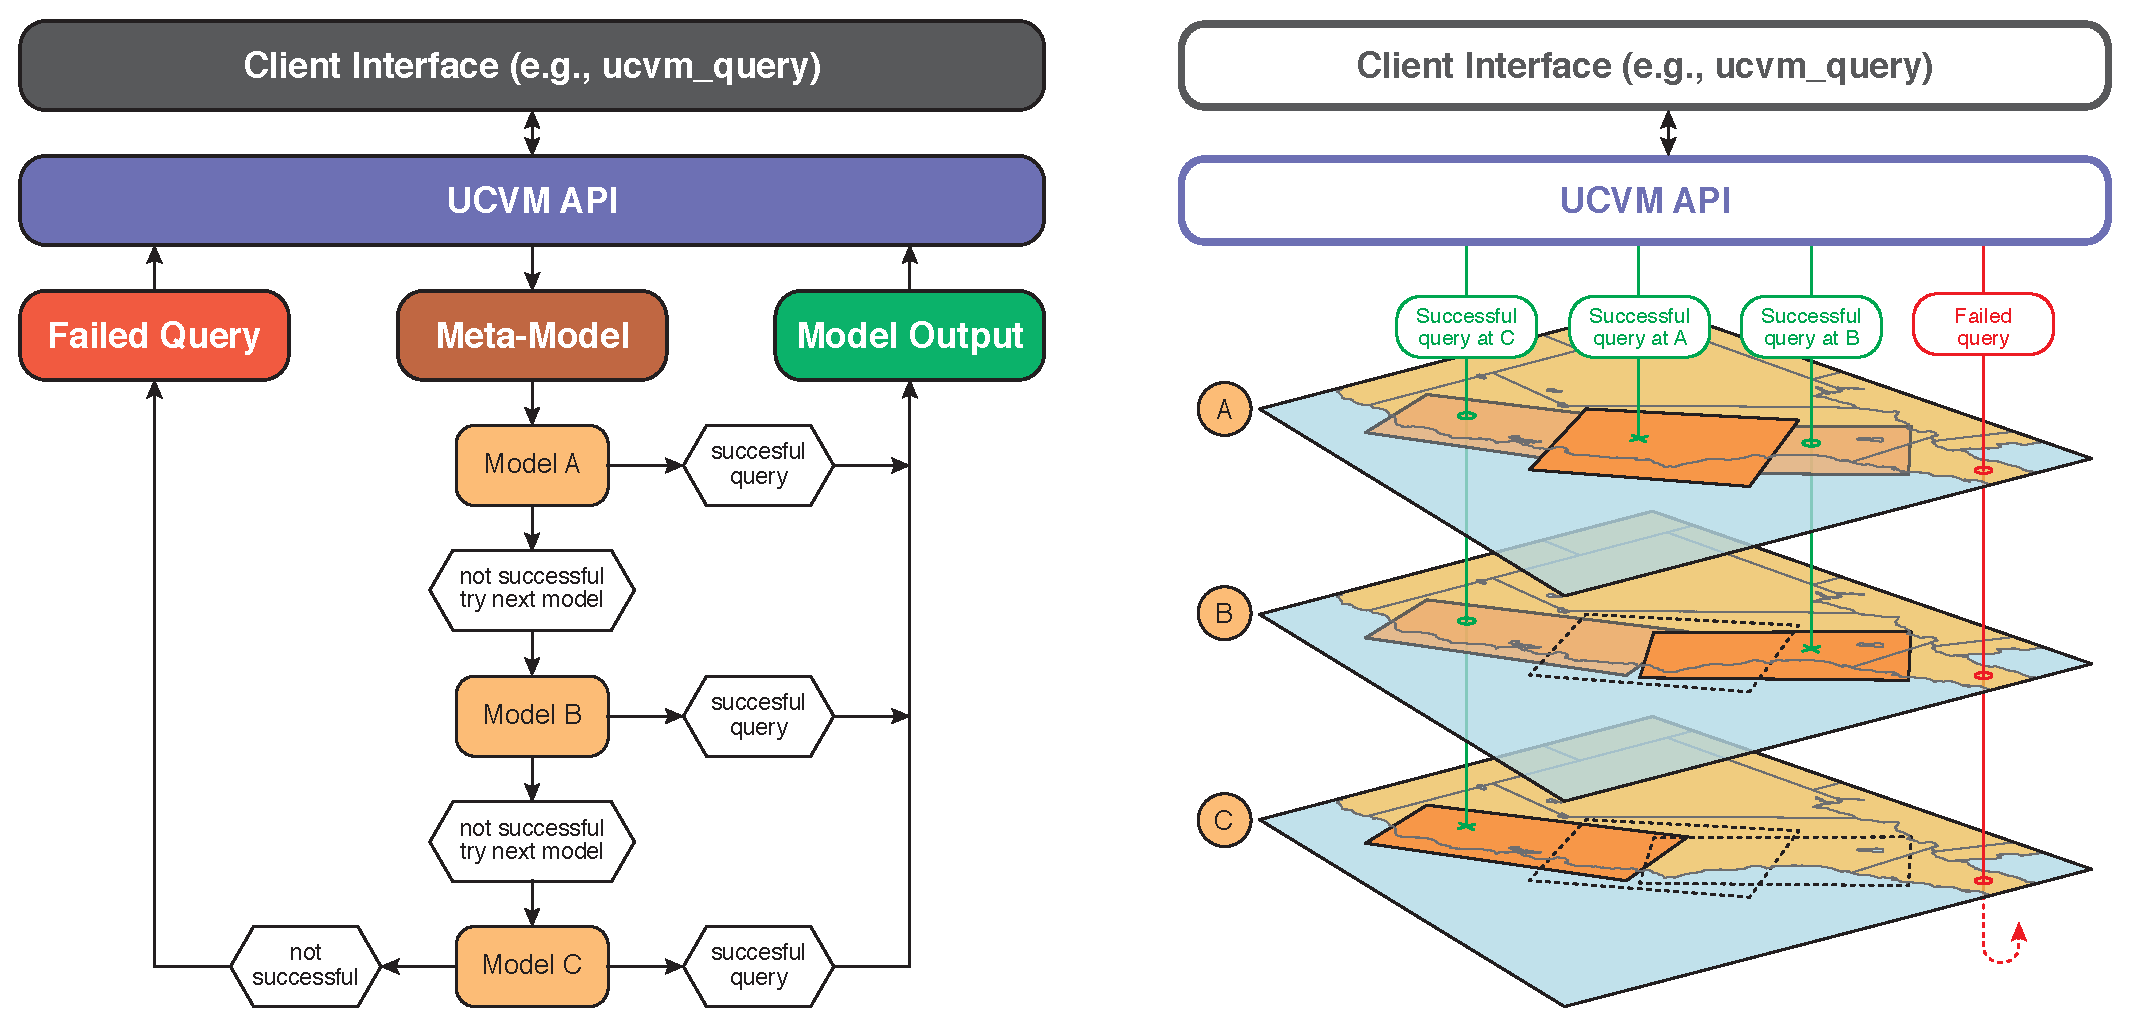
\includegraphics
		[width=0.85\textwidth]
		{figures/pdf/ucvm-query}
	\caption{UCVM querying scheme (left) and geographical illustration of the querying process (right). Information at a given geographic location is retrieved from the models registered in UCVM through a hierarchical querying scheme in which the user defines a preferred sequence of models, which are assembled internally in a meta-model. Queries to the models beneath the meta-model are carried out in the order specified by the user. Successful queried values (or failed-query results) are handled by the UCVM API wich is accessible to the user/client through a predefined interface such as the program \texttt{ucvm\_query}.}
	\label{fig:tiling}
\end{figure*}
